\section{Construction of weight coefficients set $\Q$}
\foreach \n in {1,...,16} {%
        \includegraphics[height=0.3\textheight]{img/eisenstein/phase1_image_\n.png} \hfill
        \vfill
    }

\newpage
\section{Sample of input file for shell}
File \verb+input_sample.sage+:
\label{app:inputSample}

\lstinputlisting[language=Python]{input_sample.sage}

\section{Interact in SageMath Cloud}
\label{app:interact}
\begin{figure}[!htbp]
  \centering
  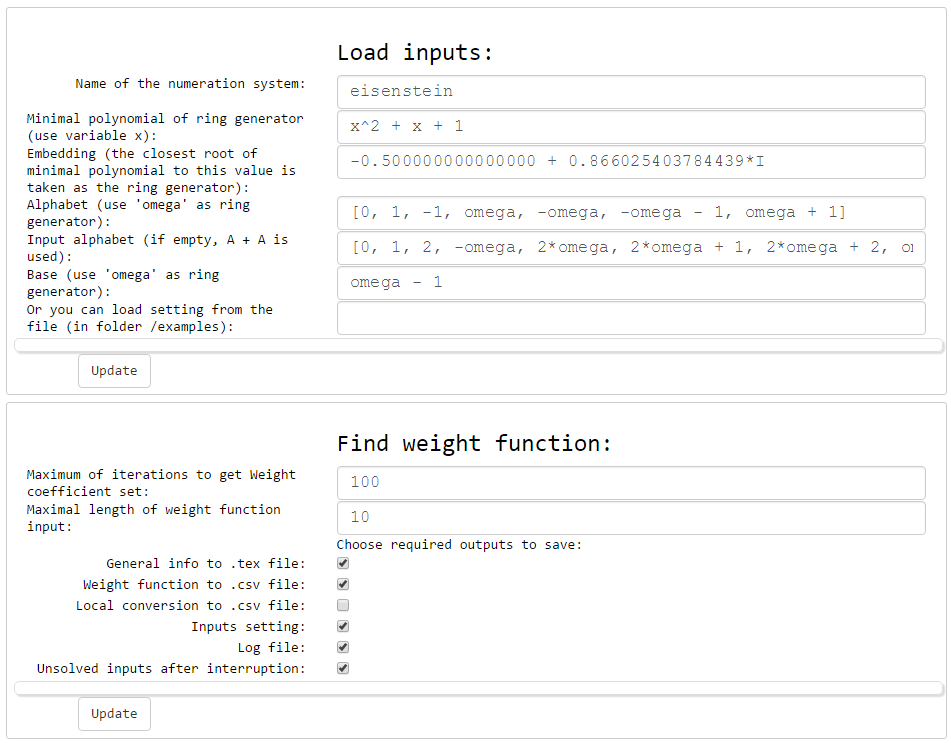
\includegraphics[width=\textwidth]{img/interact1.png}
  \caption{The interact after loading inputs.}
  \label{fig:interact1}
\end{figure}

\begin{figure}[htbp]
  \centering
  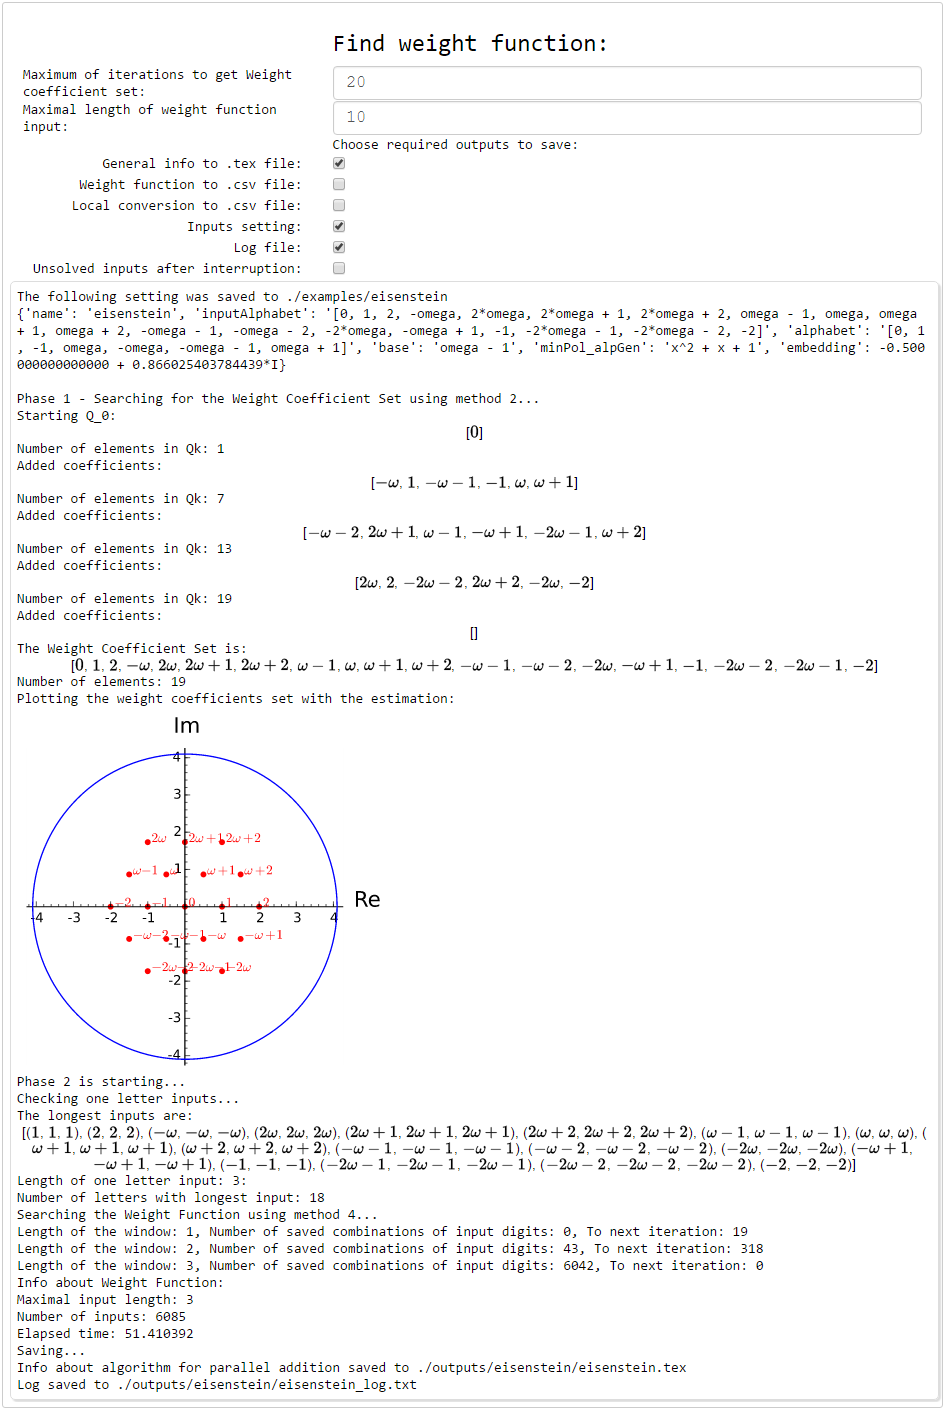
\includegraphics[width=\textwidth]{img/interact2.png}
  \caption{The output of the extending window method in the interact}
  \label{fig:interact2}
\end{figure}

\begin{figure}[htbp]
  \centering
  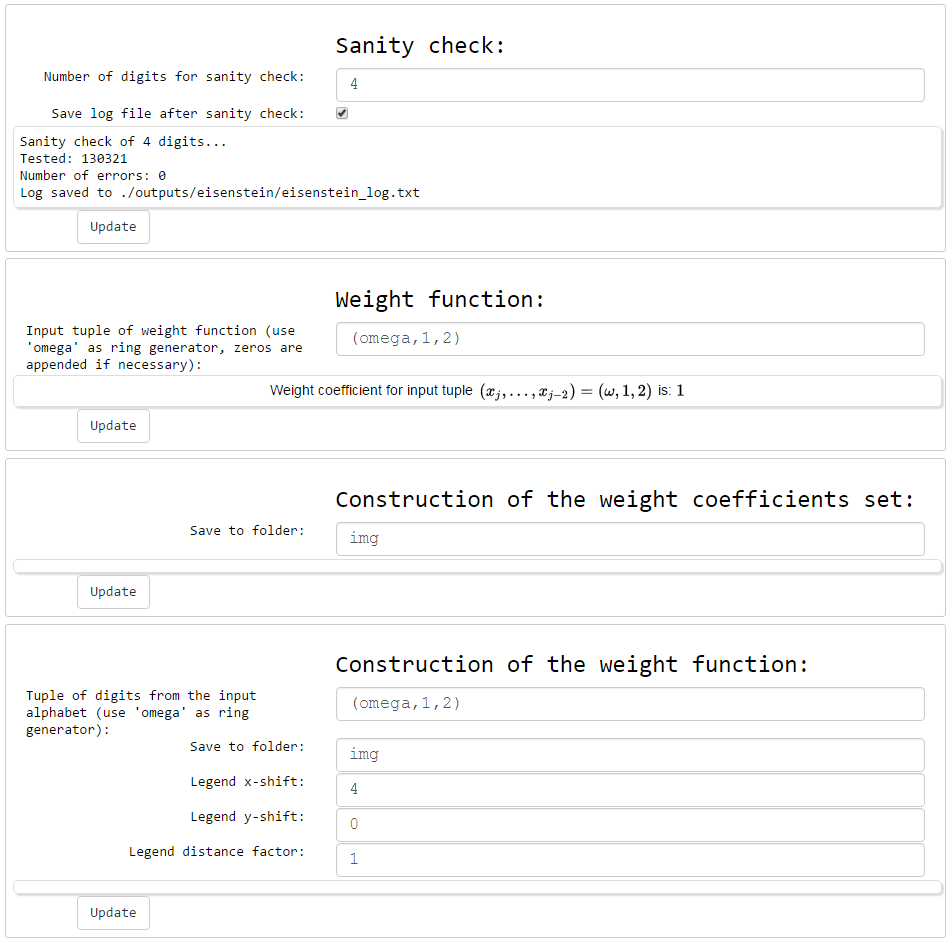
\includegraphics[width=\textwidth]{img/interact3.png}
  \caption{The part of the interact for the sanity check, calling of the weight function and plotting of images of steps of both phases.}
  \label{fig:interact3}
\end{figure}